%!TEX root = main.tex

\newpage
\subsection{수식 작성하기}
\label{subsec:ams}
드디어 \lt 의 꽃, 수식에 대해 설명을 드릴 차례입니다.
다른 어떤 편집기보다도 강력하고 편리한 수식 편집 기능을 가지고 있는 \lt 인 만큼, 실질적으로 수식 편집의 표준으로 자리 잡았기 때문에 다양한 곳에서 이제 배우는 것들을 이용할 수 있을 겁니다.
역시나 예시부터 볼까요?

\begin{Verbatim}[frame=single]
\documentclass{article}
\usepackage{kotex}
\usepackage{setspace}
\usepackage{amsmath}
\usepackage{amssymb}
\usepackage[left=2.5cm,right=2.5cm,top=3cm,bottom=3cm,a4paper]{geometry}
\begin{document}
	\doublespacing
	\noindent 수식을 입력해 봅시다.\\
	막 내용을 입력하다 중간에 짧은 수식을 넣을 수 있습니다.\\
	예를 들어 $c \in A$ 이렇게 말입니다.\\
	조금 길거나 큰 수식을 따로 입력할 수도 있습니다.\\
	예를 들어
	\[\left\{ \begin{array}{ll}
		a \in f(a)\\
		a \notin f(a)
	\end{array} \right.\]
	이렇게 말입니다.\\
	심지어
	\begin{align}
		|f(x)|=|sf_1(x)+tf_2(x)| &\le |sf_1(x)|+|tf_2(x)| \nonumber
		\\&=|s||f_1(x)|+|t||f_2(x)| \nonumber
		\\&\le |s|c_1|g(x)|+|t|c_2|g(x)| \nonumber
		\\&=(|s|c_1+|t|c_2)|g(x)| \nonumber
	\end{align}
	이런 것도 됩니다.\\
	\LaTeX 은 정말 많은 수식 요소들을 지원해줍니다.\\
	$a^{bcd}_{efg}$와 같은 첨자는 물론이고, $\sum$, $\int$같은 것도 지원합니다.
	\[\frac{\pi}{2}\]
	이렇게 분수도 잘 됩니다.
\end{document}
\end{Verbatim}
역시 바로 다음 페이지에서 결과물을 확인하실 수 있습니다.

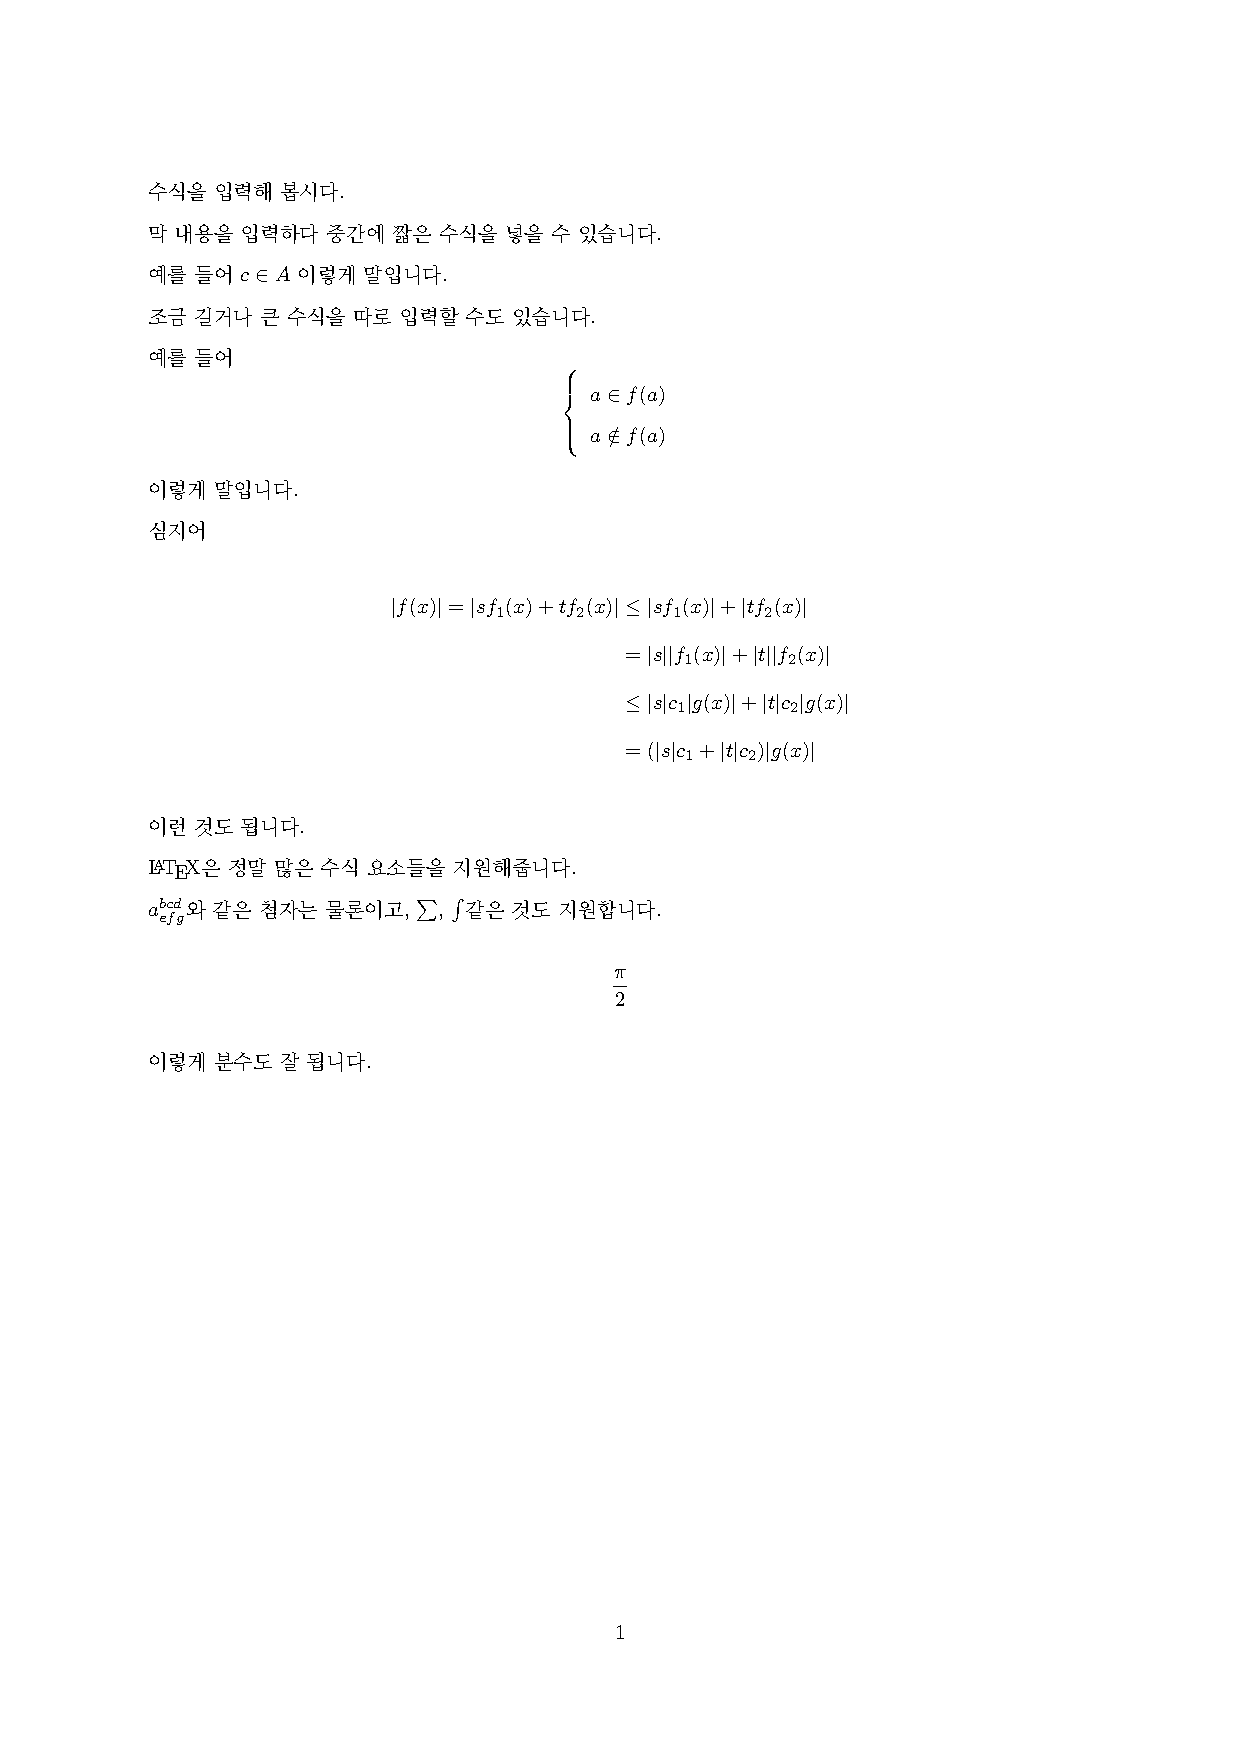
\includepdf[fitpaper=true]{example/mathexamplepdf.pdf}

예시를 잘 보면서, 천천히 시작부터 보도록 합시다.

\subsubsection{패키지 사용하기}
\label{subsec:ams-package}
보통 수식을 제대로 입력하려면 두 가지 package를 사용해야 합니다.
amsmath와 amssymb이 바로 그것들입니다.
수식을 입력해야 하는 문서라면 \verb|\usepackage{amsmath}|와 \verb|\usepackage{amssymb}|을 preamble에 입력해주세요.
참고로 한 번에 \verb|\usepackage{amsmath, amssymb}|라 쓸 수 있습니다.
수식은 웬만한 문서에 들어가기 때문에 이 한 줄을 기본적으로 입력해 두는 것을 추천합니다.
패키지를 불러왔다면, 이제 문서 어디든 수식을 입력할 준비가 된 것입니다.

\subsubsection{입력 시작하기}
\label{subsec:ams-start}
\lt 에서 수식을 입력하기 위해서는 따로 수식 편집기를 킨다거나, 그림을 추가하듯 추가하는 것이 아니라 기호 또는 command를 통해 수식을 입력함을 표시하면 됩니다.
그 방식에는 크게 세 가지 정도가 있습니다.

\paragraph{짧은 수식 삽입하기}
길고 크고 엄청난 수식을 입력하는 것이 아니라면, 보통의 경우는 수식을 문장의 중간에 넣고 싶을 겁니다.
이 때에는 내용을 입력하다가 수식을 입력하고 싶을 때 \verb|$...$|를 이용하면 됩니다.
보통 수식에서 많이 쓰이는 기호들은 저 달러 표시 안에 있어야 \lt 에서 인식할 수 있습니다.
또 저 안에 있으면 글꼴 자체가 수식에 맞도록 바뀝니다.
이 외에도 사람이 보기 좋은 수식으로 알아서 맞추어 주도록 하는 마법의 기호입니다.
다만 조금 길거나 여러 줄로 넘어가는 수식은 입력하기 어렵습니다.
꼭 일반적인 문장 중간에 넣고 싶을 때 사용해주시기 바랍니다.

\paragraph{긴 수식 삽입하기, 수식만 따로 삽입하기}
길고 크고 엄청난 수식을 입력하고 싶거나, 그래야 한다면 조금 다른 방법을 이용해야 합니다.
사실 정확히 말하자면 꼭 길지 않더라도 수식을 문장과 분리하여 따로 삽입하려면 이 방법을 이용해야 합니다.
바로 \verb|\[...\]|를 사용하는 겁니다.
이 안에 있는 모든 텍스트는 수식 입력으로 인식해서 수식으로 바꿔줍니다.
여러 행의 수식은 보통 이 방식으로 입력해줘야 하며 위의 방식보다 안정적으로 수식을 작성할 수 있습니다.
다만 이 방식 역시 모든 것이 가능한 것은 아닙니다.
그래도 웬만한 수식은 여기까지의 방법만 알아도 충분히 가능합니다.

\paragraph{특별한 수식들}
위 두 가지 방법이 아닌 다른 방법으로 수식을 입력하는 경우도 있습니다.
예시에서는 \verb|\begin{align}|이 이에 해당한다고 볼 수 있습니다.
\verb|\begin{align}|에 대한 자세한 설명은 뒤 \ref{subsec:ams-func}장에서 하도록 하겠습니다.
이 외에도 \verb|\begin{equation}|, \verb|\begin{displaymath}| 등의 수식 환경을 이용할 수 있습니다.

\paragraph{}
세 가지 방법 중 상황에 맞게 한 가지를 골라 수식을 입력하기 시작하면 됩니다.

\subsubsection{다양한 기능}
\label{subsec:ams-func}
\lt 가 수식 입력에서 그렇게 두각을 나타내고 실질적인 업계 표준이 되어 다른 편집기가 베낄 정도로 뛰어난 이유는 위에서 말씀드렸던 입력의 용이성 외에도 수식에 필요한 기능을 거의 전부 가지고 있으며 이를 미려한 디자인으로 출력해준다는 것에 있습니다.
이제 그 많은 기능들 중 자주 필요로 하는 기능들 위주로 몇가지 소개해드리려 합니다.

\paragraph{빈칸 띄우기}
수식 모드에서 단순한 빈 칸과 줄바꿈은 적용되지 않습니다.
수식에서 모든 임의로 설정하지 않은 공백은 그 수식에 맞게 알아서 설정됩니다.
이 공백을 임의로 제어하기 위해서는  \verb|\,|, \verb|\quad| 또는 \verb|\qquad|와 같은 특별한 명령으로 지정해야 합니다.
자세한 정보는 표~\ref{tab:quad}을 참조하세요.

\paragraph{글꼴 바꾸기}
수식 모드에서 모든 글자는 수식에 맞는 글꼴로 바뀌어 표현됩니다.
이 때문에 알파벳을 입력하면 이를 변수로 취급하여 변수 글꼴로 바꿔줍니다.
일반 텍스트를 수식 안에서 사용하고 싶다면 텍스트를 \verb|\textrm{...}| 안에 넣으면 됩니다.

\paragraph{그리스 문자 넣기}
수식에는 그리스 문자가 굉장히 많이 들어갑니다.
매우 보편적인 파이부터, 웬만한 그리스 문자는 한 번씩 쓰게 되죠.
\lt 은 아주 예쁜 그리스 문자들을 출력해줍니다.
물론 대문자, 소문자 모두 말입니다.
아래 그림을 참고해주세요.

\begin{figure}[h]
	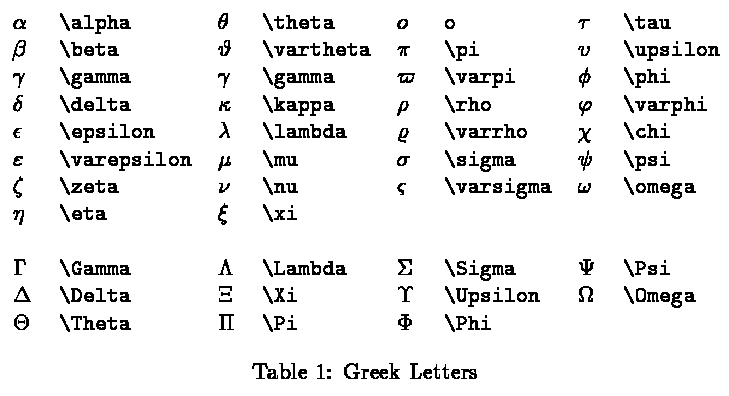
\includegraphics[width=\textwidth]{figures/t1.png}
\end{figure}

이 그림은 \url{http://web.ift.uib.no/Teori/KURS/WRK/TeX/symALL.html}에서 가져온 것으로 더 많은 정보는 직접 사이트에 들어가서 확인해주세요.

\paragraph{벡터 표시, 밑줄 등 줄긋기}
벡터를 표시하거나 선분을 표시하는 등 글자 위에 줄을 긋거나 밑줄을 쳐야 할 때가 있습니다.
벡터는 \verb|\overrightarrow{...}|와 같은 식으로 표현할 수 있습니다.
\verb|\overline{...}|처럼 그냥 선 역시 그릴 수 있습니다.
자세한 것은 표~\ref{tab:overunder}를 확인해주세요.

\paragraph{열 맞춰 쓰기}
수식을 여러 행 쓰다보면 등호와 같이 열을 맞춰 쓰고 싶을 때가 있습니다.
\verb|\begin{align}|을 사용하면 열을 맞추어 쓰고 싶은 여러행 수식을 마치 표 작성하듯 쉽게 입력할 수 있습니다.
표 작성과 방식이 굉장히 비슷하기 때문에, \ref{subsec:tabfig}장을 미리 보고 익히셔도 좋습니다.
방식을 설명해드리자면, 먼저 예시를 봅시다.
예시에서 볼 수 있듯 등호, 부등호 처럼 같은 열에 맞춰 쓰고 싶은 기호들 앞에 공통된 기호를 하나 입력했습니다.
\verb|&|입니다. 이 기호는 표에서도 비슷한 역할을 하므로 기억해 둡시다.
즉 같은 열에 맞추어 쓰고 싶은 부분 바로 앞에 \verb|&|를 붙이고, 줄바꿈은 아시는 대로 \verb|\\|를 이용하시면 됩니다.

\paragraph{여러 줄 묶기}
혹은 대괄호로 여러 행의 식을 묶어 표현해야 할 때도 있습니다.
여러 개의 식으로 정의되는 함수를 표현한다거나 할 때, 큰 중괄호로 식들을 묶는 방식을 많이 보셨죠?
바로 그것을 쉽게 표현할 수 있다는 겁니다.
예시에도 나와 있듯이 \verb|\[\]| 안에 \verb|\begin{array}{...}|를 이용하는 방법입니다.
이 환경 역시도 표 작성 방식과 거의 일치합니다.
구체적이고 자세한 것은 역시나 \ref{subsec:tabfig}장을 먼저 읽어서 이해하시는 것을 추천드립니다.
간략히 설명을 드리자면, \dots 에는 묶고 싶은 수식의 열과 각 열의 정렬 방식에 따라 알맞은 문자를 넣습니다.
array 환경 앞에는 \verb|\left|, 그리고 중괄호와 같이 묶는 데 쓸 기호를 입력합니다.
array 환경 안에서 묶을 식들을 예시와 같이 입력하고, array 환경이 끝나고 \verb|\right.|을 입력하면 됩니다.

이 외에도 정말 수많은 기능과 command들이 존재합니다.
수식 기호 관련한 command 및 문법 정보는 위키피디아의 TeX 문법\footnote{\url{https://en.wikipedia.org/wiki/Help:Displaying_a_formula}} 문서를 확인하면 대부분 찾을 수 있습니다.

\newpage
\subsection{표와 그림}
\label{subsec:tabfig}
이제 거의 다 왔습니다. 초 입문서의 끝이 보입니다.\\
이번에는 표와 그림을 삽입하는 방법에 대해서 알아봅시다.
표와 그림은 \lt 환경에서 `떠다니는 개체'라는 개념으로 이해됩니다.
이는 표, 그림등으로 된 하나의 개체가 떠다니듯 존재해 그 위치를 일정한 규칙에 맞춰 유동적으로 결정한다는 의미라고 보시면 됩니다.\\
언제나처럼 예시부터 볼까요?

\begin{Verbatim}[frame=single]
	\documentclass{article}
	\usepackage{kotex}
	\usepackage{setspace}
	\usepackage[pdftex]{color, graphicx}
	\usepackage[left=2.5cm,right=2.5cm,top=3cm,bottom=3cm,a4paper]{geometry}
	\begin{document}
	\doublespacing
	\noindent 이번에는 표와 그림에 대해서 봅시다.\\
	먼저 표는 이렇게 그리면 됩니다.
	\begin{table}[hp]
	\centering
	\begin{tabular}{|c|c|}
	\hline
	그냥 & 이런\\
	\hline
	식으로 & 하면\\
	\hline
	표가 & 됩니다\\
	\hline
	\end{tabular}
	\caption{캡션은 이렇게 답니다}
	\label{tab:eg}
	\end{table}
	참 쉽죠?\\
	다음은 그림입니다.
	\begin{figure}[hp]
	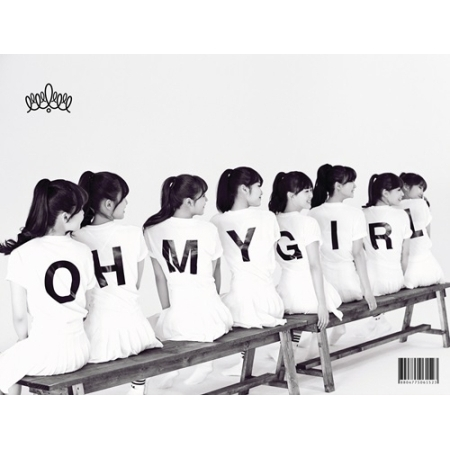
\includegraphics[width=0.9\textwidth]{OhMyGirl.jpg}
	\caption{그림도 캡션이 됩니다}
	\label{fig:eg}
	\end{figure}
	\end{document}
\end{Verbatim}

결과는 다음 페이지에서 확인하시면 됩니다.

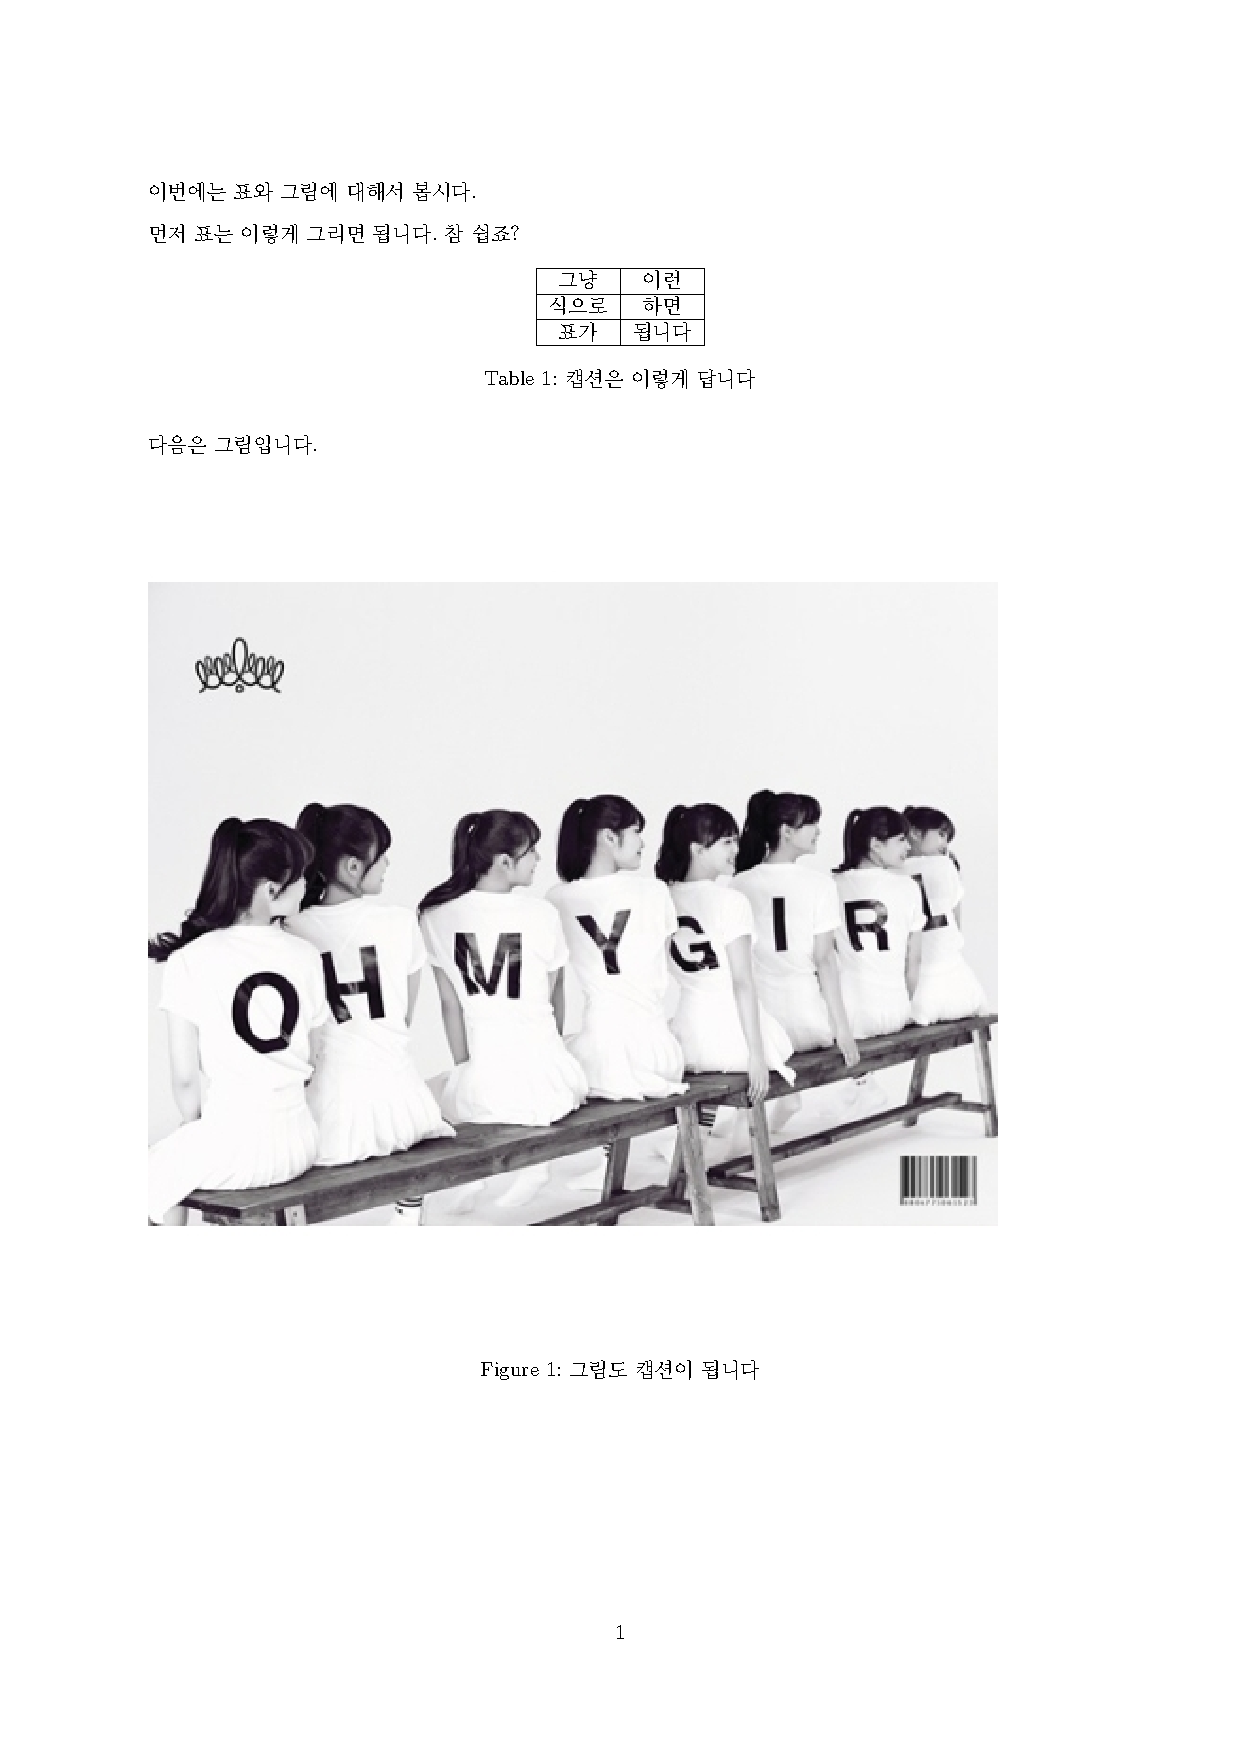
\includepdf[fitpaper=true]{example/tabfigexample.pdf}

그럼 각각 어떤 식으로 삽입하는지 이제부터 알아보도록 합시다.

\subsubsection{표}
\label{subsec:mktab}
먼저 표부터 살펴봅시다.
표를 삽입하는 것은 두가지 절차로 나누어 생각하면 쉽습니다.
표를 그리기 위한 과정과 표를 일정한 위치에 삽입하기 위한 과정이 그 절차들입니다.
절차를 나눠 천천히 익혀봅시다.

\paragraph{표 그리기}
표를 그리는 데에는 \verb|\begin{tabular}{pos}|를 이용하면 됩니다.
여기서 pos 에 들어가는 것은 위의 수식 입력하기에서 array 환경에서도 봤던 바로 그것입니다.
표의 형태를 미리 정의하는 과정인데, 표가 몇 열로 이루어지는지, 각 열은 어떤 정렬로 할지, 각 열 사이 세로선은 넣을지 말지 결정할 수 있습니다. 예시에서는 $\mid$c$\mid$c$\mid$ 라고 되어 있군요.
여기서 $\mid$는 세로선을 의미하고 각 알파벳은 하나의 열을 뜻합니다.
특히 c는 center, 즉 가운데 정렬을 의미합니다.
이런 식으로 표의 형태를 어느 정도 결정해주는 겁니다.
pos에 들어가는 글자들에 대한 전체 정보는 표~\ref{tab:pos}를 참고해주세요.
pos까지 결정했다면 표를 그리기 시작하면 됩니다.
각 열은 \verb|&|로, 각 행은 \verb|\\|로 구분하여 작성합니다.
가로줄을 원한다면 각 행 사이에 \verb|\hline|을 입력하면 됩니다.
열 병합을 원한다면 \verb|\multicolumn{number}{pos}{text}|을 이용하세요.
number엔 병합할 열 개수, pos는 새로 병합한 열의 형태, text엔 내용을 입력하면 됩니다.

\paragraph{표 삽입하기}
표를 다 그리셨으면 문서에 삽입을 해야겠죠?
예시를 봅시다. tabular 환경을 감싸고 있는 것이 있습니다.
\verb|\begin{table}[pos]|입니다.
그려진 표를 위치시키기 위한 환경입니다.
이 환경에서도 pos가 있습니다.
여기서 pos는 표의 위치를 결정하는 부분입니다.
h, p, t, b, !로 이루어집니다.
여기서 h는 당장 입력하고 있는 바로 그곳을 뜻합니다.
p는 새로운 페이지를 뜻합니다. 다시 말해 떠다니는 개체가 모이는 특정 페이지를 뜻합니다.
t는 페이지 맨 위를 뜻합니다.
b는 페이지 맨 아래를 뜻합니다.
!는 개체를 위치시키는 일정한 규칙을 무시하고 선언한 대로 위치하도록 강제한다는 뜻입니다.
대신 개체, 즉 표가 출력 과정에서 아예 위치되지 못할 수도 있습니다.
이 문자들을 이용하여 '!hbp'와 같은 식으로 표를 위치시킬 방법을 선언합니다.
!hbp라면 기존 규칙을 무시하고 당장 입력하고 있는 곳에 위치시키거나, 그게 불가능하면 페이지 맨 아래에 위치시키거나, 그것도 불가능하면 새 페이지에 위치시키겠다는 말입니다.\\
table 환경에서는 \verb|\centering|으로 표를 가운데에 위치시킬 수도 있습니다.
또 tabular로 표 작성이 끝난 뒤 table환경이 끝나기 전에 \verb|\caption{text}|으로 캡션을 달 수도 있습니다.
표를 참조하고 싶다면 캡션 command 바로 뒤에서 \verb|\label{}|을 이용하면 됩니다.

\paragraph{}
이정도만 익히면 웬만한 표들은 작성이 가능할겁니다.

\subsubsection{그림}
\label{sec:advanced_2-pic}
이제 그림을 넣어봅시다.
그림은 초 입문자 분들께서는 package의 사용이나 그 과정이 이해되기 힘들겁니다.
확장자가 eps냐 다른 것이냐에 따라 컴파일 과정이 달라지고, package도 조금씩 바꿔서 써야 합니다.
일단 여기서는 보편적으로 쓰이는 일반 확장자들에 대한 방법 위주로 설명을 드리겠습니다.

\paragraph{package 사용하기}
png, jpg, pdf, mps 확장자를 가지는 그림 파일들은 packge의 사용을 필요로 합니다.
\verb|\usepackage[pdftex]{color,graphicx}|를 이용합시다.
예시에도 잘 나와 있는 이 package를 이용해야 앞에서 말씀드린 확장자의 그림 파일들을 삽입할 수 있습니다.
뒤에서 그림을 삽입할 때 사용하는 command를 설명해드릴건데, 당연하지만 이 command에는 삽입하려는 그림 파일 이름을 입력해야 합니다.

\paragraph{그림 삽입하기}
이제 정말 그림을 넣어봅시다.
그림도 어떻게 보면 표처럼 두 가지 절차로 나누어집니다.
그림을 불러오는 과정과 위치시키는 과정입니다.\\
먼저 불러오는 과정은 \verb|\includegraphics[key=value...]{imagefile}|를 이용하면 됩니다.
key에는 height, width등이 들어가며, 각 key의 value를 고정시켜줄 수 있습니다.
예를 들어, \verb|width=0.5\textwidth|라고 해주면 그림의 가로 길이를 문단 가로 길이의 0.5배로 고정시킨다는 뜻이 되는 겁니다.
imagefile에는 파일명을 입력하시면 됩니다.

\paragraph{그림 위치시키기}
다음으로 위치시키는 과정은 기본적으로 위의 table 환경 설명에서 table 대신 figure를 입력하면 됩니다.
조금 더 자세히 다시 설명해드리자면, 그림을 위치시키기 위해 \verb|\begin{figure}[pos]|를 이용한다는 것입니다.
여기서 pos는 table에서와 마찬가지로 h, p, b, t, !로 이루어집니다.\\
또한 \verb|\includegraphics[key=value]{imagefile}| 뒤에 캡션과 라벨 역시 사용할 수 있도록 해줍니다.

\paragraph{심화 기능들}
여기서 조금 더 심화적인 기능을 써볼까요?
지금까지의 방법으로는 그림은 새로운 줄 혹은 페이지에 위치해 자리 차지를 엄청 크게 합니다.
마이크로소프트 워드에서 `위/아래'라고 되어 있는 레이아웃에 해당한다는 말입니다.
그림을 텍스트가 둘러싸게 위치시키고 싶을 때가 많을 겁니다.
마이크로소프트 워드에서 `정사각형'이라고 되어 있는 레이아웃에 해당하도록 할 수 있다는 겁니다.\\
일단 \verb|\usepackage{wrapfig}|를 preamble에 추가해줍니다.\\
그리고 그림을 위치시키고 싶을 때 \verb|\begin{wrapfigure}{pos}{width}}|를 이용하면 됩니다.
여기서 말하는 pos는 문단의 오른쪽에 위치시킬지 왼쪽에 위치시킬지 결정하는 부분입니다.
왼쪽은 l 또는 L, 오른쪽은 r 또는 R을 입력하면 됩니다.
width에는 말 그대로 그림을 넣을 자리의 가로 길이를 설정하는 부분입니다.
주의하세요. 그림의 가로 길이가 아닙니다.
그림을 넣을 자리의 가로 길이입니다.\\
이번에는 한 줄에 여러 개의 그림을 넣어봅시다.
역시나 package를 추가해야 합니다.\\
\verb|\usepackage{subcaption}|을 추가해줍니다.
그 다음은 쉽습니다.
기본적으로 그림을 위치시킬 때 쓰는 figure 환경 안에서, 넣고 싶은 그림마다 \verb|\begin{subfigure}{width}|를 써주면 됩니다.
width에는 역시나 각 그림이 들어갈 자리의 가로 길이를 써주면 됩니다.
물론 각 그림 하나하나마다 캡션을 달고 참조시킬 수 있습니다.
figure 환경에서 캡션 달듯이 subfigure에 달면 됩니다.

\paragraph{}
역시나 이정도만 알고 계신다면 일반적인 그림 파일들은 삽입할 수 있을 겁니다.

\subsection{문제가 생기셨나요?}
\label{subsec:problem4}
물론 수식을 작성하실 때, 표나 그림을 삽입하실 때에도 문제는 발생할 수 있습니다.
어떤 문제가 생기든 겁먹지 마세요.
문제를 해결하기 위해 다시 돌아왔습니다.
지금부터 하나하나 짚어봅시다.
\begin{itemize}
	\item \verb|align|환경을 이용하실 때 원하는 모양대로 안 나오거나 에러가 떴나요?
	혹시 줄바꿈을 제대로 해주었는지 확인해보세요.
	열을 맞추기 위해 \verb|&|를 입력하고 나면 그 다음 \verb|&|이 나오기 전에 꼭 줄바꿈을 해줘야 합니다.

	\item 수식 모드에서는 텍스트 모드와 달라 주의할 점들이 많습니다.
	특히 공백 문자는 전부 무시해버린다는 사실은 꼭 기억해두고 본문에서 설명드린 강제 공백 명령어들을 이용해주세요.
	다만 \lt 에서 강제로 디자인에 영향을 주는 것은 언제 어떤 문제가 생길지 모르는 행동입니다.
	너무 남용하지는 말아주세요.
	
	\item 수식 모드의 공백 기호에서 반각은 \verb|\| 입니다.
	그냥 역슬래시 하나라 굉장히 당황스럽겠지만, 모든 명령어가 그렇듯 역슬래시 하나만 입력하고 스페이스 혹은 중괄호와 같은 비문자를 입력해주면 됩니다.
	
	\item 반대로 텍스트 모드이기 때문에 수식 모드와 구분해야 하는 경우도 있습니다.
	생각보다 많은 부호, 기호들이 텍스트 모드에서는 동작하지 않습니다.
	$\mid$ 같은 기호들은 전부 수식 모드 안에서만 동작하죠.
	이 점 유의해주세요.
	만약 에디터로 \TeX Studio를 사용하고 계신다면 더더욱 주의해주세요.
	쓸 수 있는 명령어들의 자동완성 기능은 이 에디터의 특장점이지만 텍스트 모드에서 쓸 수 없는 수식 모드 전용 명령어들까지 텍스트 모드에서 자동완성 시켜줍니다.
	자동완성 된다고 안심하지 마세요.
	
	\item 표나 그림에 캡션을 달고 그 캡션에 label을 달게 되는 경우가 많습니다.
	이 때 주의할 점이 있습니다.
	꼭 \verb|\caption{text}| 뒤에 \verb|\label{text}|을 입력해주세요.
	순서가 바뀌면 번호가 잘못 매겨지는 경우가 간혹 있습니다.
	
	\item 조금 전에 \lt 환경에서 강제로 디자인에 영향을 주는 것이 좋지 못한 행동이라고 말씀을 드렸습니다.
	이것이 정말 크게 드러나는 부분이 표, 그림에서 위치선정 부분입니다.
	`떠다니는 개체'라고 불리는 표, 그림은 그 이름 만큼이나 자유롭고 유동적으로 위치가 결정됩니다.
	만약 별일이 없다면 \lt 에서 일정한 규칙에 맞게 배치를 해줍니다.
	그런데 table이나 figure 환경에서 !를 사용한다거나, 어떻게든 사용자가 원하는 자리에 두기 위해서 다양한 실험을 하는 분들이 계실 겁니다.
	이런 행동, 정말 주의하셔야 합니다.
	본문에서 설명 드렸듯이 !를 사용하다가는 \lt 이 개체를 배치할 자리를 못 찾고 아예 삽입이 안 될 수도 있습니다.
	또 원하는 자리에 두기 위한 지나친 노력은 대부분 에러, 워닝, 배드박스를 부르는 원인이 됩니다.
	\lt 의 자리 배정 규칙을 믿고, 어느 정도는 유연하게 받아들이는 것이 상책입니다.
	그게 어쩌면 제일 예쁠지도 몰라요.
	
	\item 그림을 넣으실 때 파일 확장자까지 입력해주지 않는다면 아주 약간의 문제가 생길 수 있습니다.
	당장은 문제가 없어보일 수도 있지만 확장자까지 꼭 적어주시기 바랍니다.
	참고로, eps 확장자의 그림 파일을 삽입하고 싶다면 package의 pdftex 부분을 driver로 바꿔주거나, 확장자를 입력하지 않으면 됩니다.
	역시나 전자의 방법을 추천드립니다.
	
	
\end{itemize}
여기에 없는 문제들은 친구에게 물어보거나, 구글에 검색해 보세요. 아마 여러분과 같은 어려움을 겪고 있는 사람들이 상당히 많을 겁니다.


%%% Local Variables:
%%% mode: latex
%%% TeX-master: "main"
%%% End:
